\documentclass[table,xcolor=dvipsnames,professionalfonts]{beamer}
\usepackage{xcolor}
\usepackage{booktabs}
\usepackage{graphicx}
\usepackage{tikz}
\usepackage{feynmp}
\usepackage{xspace}
\usepackage{slashed}
%\usepackage[utopia]{mathdesign}
\usepackage[charter]{mathdesign}
\usepackage[UKenglish]{babel}
\usepackage[utf8]{inputenc}
%\usepackage{lmodern}
\setbeamertemplate{navigation symbols}{}
\usepackage{appendixnumberbeamer}
%\usepackage{hepparticles}
%\usepackage{hepnicenames}
\usepackage{hepunits}
\usepackage{bbm}

\ifpdf
\usepackage{epstopdf}
\usepackage[protrusion=true,expansion=true,tracking]{microtype}
%\DeclareGraphicsRule{*}{mps}{*}{}
\fi

\usepackage{listings}
\usepackage[framemethod=tikz]{mdframed}
\lstloadlanguages{C++}
\makeatletter
\newcommand{\srcsize}{\@setfontsize{\srcsize}{5pt}{5pt}}
\makeatother
\lstset{language=[11]C++,
  literate= % define some ligatures for PragmataPro
  {!!}{\texttt{!!}}2 {::}{\texttt{::}}2 {++}{\texttt{++}}2
  {--}{\texttt{--}}2 {()}{\texttt{()}}2 {\[\]}{\texttt{[]}}2
  {==}{\texttt{==}}2 {!=}{\texttt{!=}}2 {>=}{\texttt{>=}}2
  {<=}{\texttt{<=}}2 {&&}{\texttt{\&\&}}2 {||}{\texttt{||}}2
  {!>}{\texttt{!>}}2 {\#(}{\texttt{\#(}}2 {\#_}{\texttt{\#_}}2
  {\#\{}{\texttt{\#\{}}2 {\#?}{\texttt{\#?}}2 {\#>}{\texttt{\#>}}2
  {\%=}{\texttt{\%=}}2 {+=}{\texttt{+=}}2 {-=}{\texttt{-=}}2
  {*=}{\texttt{*=}}2 {/=}{\texttt{/=}}2 {&=}{\texttt{&=}}2
  {^=}{\texttt{^=}}2 {|=}{\texttt{|=}}2 {~=}{\texttt{~=}}2
  {<<}{\texttt{<<}}2 {>>}{\texttt{>>}}2 {->}{\texttt{->}}2
  {__}{\texttt{\_\_}}2
  {!!!}{\texttt{!!!}}3 {>>=}{\texttt{>>=}}3 {<<=}{\texttt{<<=}}3
  {/==}{\texttt{/==}}3 {...}{\texttt{...}}3,
  deletekeywords=[1]{auto,const,static,volatile,void,char,short,int,long,unsigned,float,double,inline,template,typename,namespace,class,union,struct,enum,true,false,nullptr},
  morekeywords=[2]{auto,const,static,volatile},
  morekeywords=[3]{void,char,short,int,long,unsigned,float,double,size_type,inline,iterator,const_iterator,reference,const_reference,Uninitialised,template,typename,namespace,class,union,struct,enum},
  morekeywords=[4]{std,our,LHCb,T,ARGS},
  morekeywords=[5]{true,false,nullptr,__LINE__,__FILE__,__func__},
  basicstyle=\srcsize\ttfamily\color{black},
  keywordstyle=[1]\color{magenta}\textbf,
  keywordstyle=[2]\color{orange}\textbf,
  keywordstyle=[3]\color{cyan}\textbf,
  keywordstyle=[4]\color{black},
  keywordstyle=[5]\color{violet!80!white},
  directivestyle=\color{blue!50!white},
  commentstyle=\color{blue}\textsl,
  stringstyle=\color{gray},
  identifierstyle=\color{green!50!black},
breaklines=true,breakautoindent=true}

\mdfdefinestyle{listing}{
  backgroundcolor=white!96!black,hidealllines,
  skipabove=0pt,skipbelow=0pt,
  leftmargin=0pt,rightmargin=0pt,
  innertopmargin=-5pt,innerbottommargin=-5pt,
  innerleftmargin=0pt,innerrightmargin=0pt,
  linewidth=0pt,middlelinewidth=0pt,
  startcode={\vspace{-3pt}},endcode={\vspace{-2ex}}
}
\surroundwithmdframed[style=listing]{lstlisting}

\usepackage{fontspec}
%\setmainfont{CharisSIL}[]
%\setsansfont{FrontPagePro}[Scale=MatchLowercase]
\setmonofont{PragmataPro}[Scale=MatchLowercase]

\usetheme{Rochester}
%\usecolortheme{beaver}
\usecolortheme[named=NavyBlue]{structure}
\setbeamercolor{section in toc}{fg=black,bg=white}
%\setbeamercolor{alerted text}{fg=blue}
\setbeamercolor{structure}{fg=blue!80!black}
\setbeamercolor*{palette primary}{fg=black,bg=gray!30!white}
\setbeamercolor*{palette secondary}{fg=black,bg=gray!15!white}
\setbeamercolor*{palette tertiary}{bg=blue!80!black,fg=gray!10!white}
\setbeamercolor*{palette quaternary}{fg=blue,bg=gray!5!white}
\setbeamercolor*{sidebar}{fg=blue,bg=gray!15!white}
\setbeamercolor*{palette sidebar primary}{fg=blue!10!black}
\setbeamercolor*{palette sidebar secondary}{fg=white}
\setbeamercolor*{palette sidebar tertiary}{fg=blue!50!black}
\setbeamercolor*{palette sidebar quaternary}{fg=gray!10!white}
\setbeamercolor{titlelike}{parent=palette primary,fg=blue,bg=white}
\setbeamercolor{frametitle}{fg=white,bg=blue!80!black}
\setbeamercolor{frametitle right}{bg=gray!60!white}
\setbeamercolor*{separation line}{}
\setbeamercolor*{fine separation line}{}
\useinnertheme{rectangles}
\useoutertheme{infolines}
\usefonttheme[onlymath]{serif}
%\usefonttheme{professionalfonts}

%\loadgraphics{logo-pi-bunt3,lhcb-logo,unisiegel-gray}

\newsavebox{\unilogo} \newsavebox{\pilogo} \newsavebox{\lhcblogo}
\sbox{\unilogo}{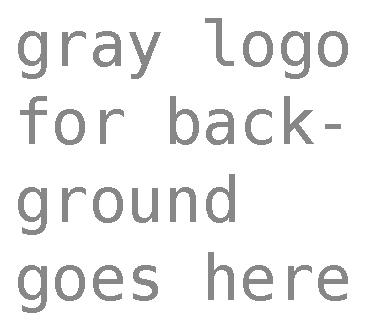
\includegraphics[height=1.2cm]{../cern-logo-gray.eps}}
\sbox{\pilogo}{
\includegraphics[height=0.75cm]{../cern-logo.eps}}
\sbox{\lhcblogo}{
\includegraphics[height=0.75cm]{../lhcb-logo.eps}}

\setbeamertemplate{footline}
{
  \leavevmode%
  \hbox{%
    \begin{beamercolorbox}[wd=.333333\paperwidth,ht=2.25ex,dp=1ex,left]{author in head/foot}%
      \usebeamerfont{author in head/foot}\vtop{\vskip-2.25ex\hbox{\resizebox{!}{3.25ex}{\usebox{\pilogo}}}}%
      \hfill \insertshortauthor~~(\insertshortinstitute) \hfill%
    \end{beamercolorbox}%
    \begin{beamercolorbox}[wd=.333333\paperwidth,ht=2.25ex,dp=1ex,center]{title in head/foot}%
      \usebeamerfont{title in head/foot}\insertshorttitle%
    \end{beamercolorbox}%
    \begin{beamercolorbox}[wd=.333333\paperwidth,ht=2.25ex,dp=1ex,right]{date in head/foot}%
      \usebeamerfont{date in head/foot}\insertshortdate{}\hspace*{2em}%
      \insertframenumber{} / \inserttotalframenumber\hspace*{2ex} \vtop{\vskip-2.25ex\hbox{\resizebox{!}{3.25ex}{\usebox{\lhcblogo}}}}%
    \end{beamercolorbox}%
  }%
  \vskip0pt%
}

\setbeamertemplate{frametitle}
{
  \ifbeamercolorempty[bg]{frametitle}{}{\nointerlineskip}%
  \leavevmode%
  \vskip-2pt\hbox{%
    \begin{beamercolorbox}[wd=\paperwidth,left]{frametitle}%
      \usebeamerfont{frametitle}%
      \vskip.125ex%
      \hbox{\vtop{\raisebox{-1ex}[1ex][1ex]{\makebox[0pt][l]{\usebox{\unilogo}}}%
      \hspace{1em}\strut\insertframetitle\strut}\par%
      {%
        \ifx\insertframesubtitle\@empty%
        \else%
        {\usebeamerfont{framesubtitle}\usebeamercolor[fg]{framesubtitle}\insertframesubtitle\strut\par}%
        \fi
      }}%
    \end{beamercolorbox}%
  }%
}


\definecolor{bandgreen}{rgb}{0.4,0.8,0.4}
\newcommand{\FIXME}{{\color{red}FIXME}}
\newcommand{\arxiv}[1]{{\color{gray}\tiny$[$\href{http://arxiv.org/abs/#1}{arXiv:#1}$]$}}
\newcommand{\jref}[2]{{\color{gray}\tiny$[$\href{#2}{#1}$]$}}
\newcommand{\myhref}[2]{\href{#1}{\textcolor{blue}{#2}}}


\author[Paul Seyfert]{Paul Seyfert}
\institute[CERN]{CERN}
\date[\today]{VERTEX 2017}
\title[LHCb upgrade]{Tracking, Vertexing and data handling strategy for the LHCb upgrade}


\begin{document}
\maketitle

\begin{frame}
  \frametitle{scope I}

  \begin{columns}
    \begin{column}{.65\textwidth}
      \begin{center}
%\uselengthunit{mm}\printlength{\textwidth}.
        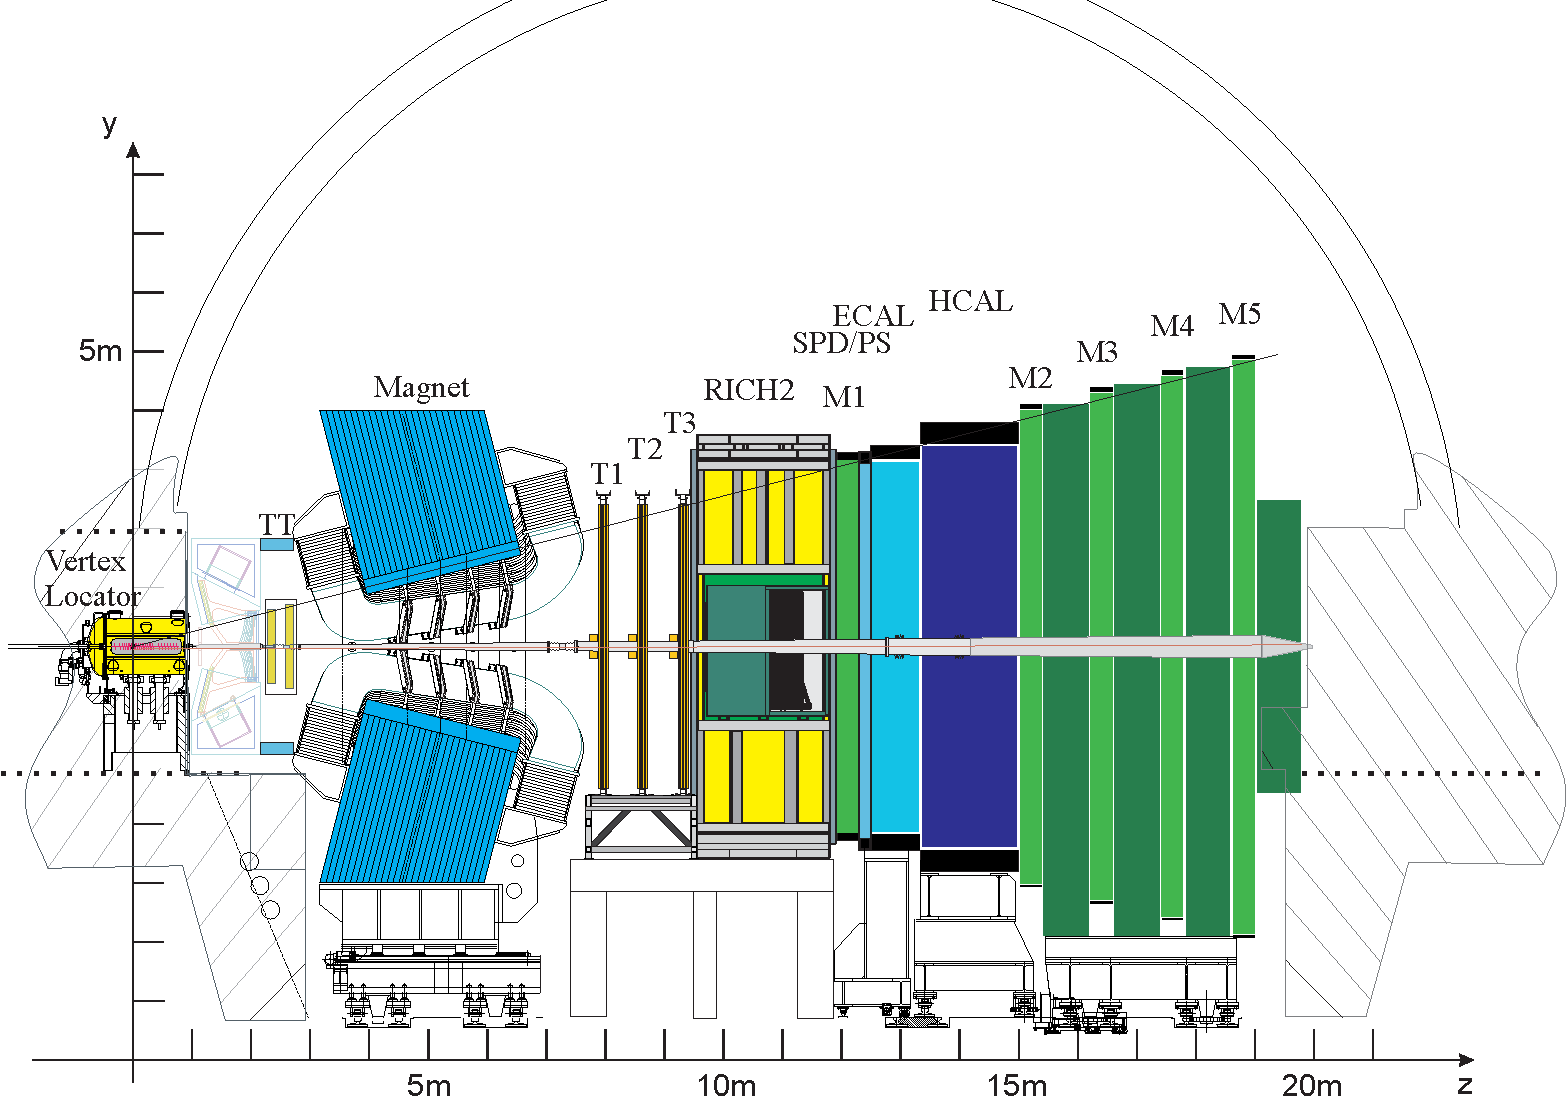
\includegraphics[width=0.92\textwidth,trim=0 0 0 50,clip]{/home/pseyfert/phd/talks/irtg20120615/LHCb-reoptimized-y.pdf}
        \hspace{-0.92\textwidth}
        \resizebox{0.92\textwidth}{!}{
          \begin{tikzpicture}
            \useasboundingbox (0,0) rectangle (752pt,476pt);
          \end{tikzpicture}
        }
      \end{center}
    \end{column}
    \begin{column}{.35\textwidth}
      \begin{itemize}
        \item Fully equipped forward detector at the LHC
        \item Approaching 400 papers
        \item exceeding our own expectations:
          \begin{itemize}
              \item online calibration and alignment
              \item exceeding design pile-up
          \end{itemize}
      \end{itemize}
    \end{column}
    \end{columns}
    \end{frame}

    \begin{frame}
      \frametitle{scope II}
      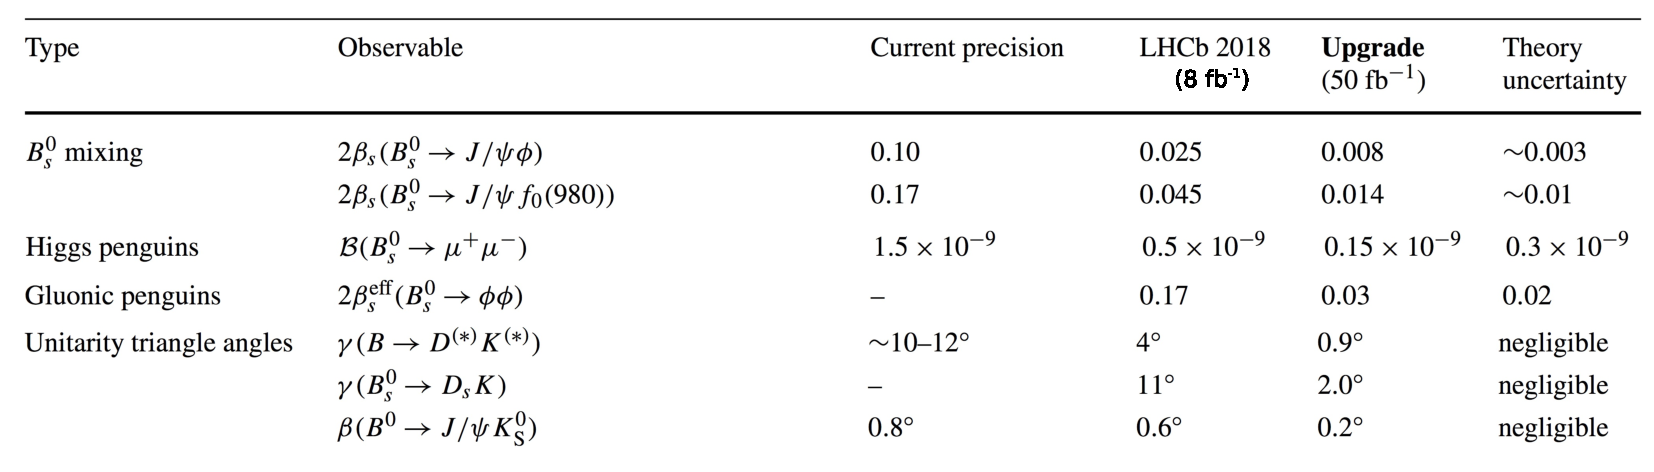
\includegraphics[width=\textwidth]{./alessiotable.pdf}

      {\footnotesize{\texttt{Eur. Phys. Journal C (2013) 73:2373}}}

      \begin{itemize}
          \item By 2018 important analyses will still be statistically limited
          \item Theoretical uncertainty smaller than experimental
          \item[$\rightarrow$] Significantly more statistics needed
          \item[$\Rightarrow$] Go to higher luminosity
      \end{itemize}
    \end{frame}


\begin{frame}
  \frametitle{removal of hardware trigger I}
  \begin{columns}
  \begin{column}{.6\textwidth}
    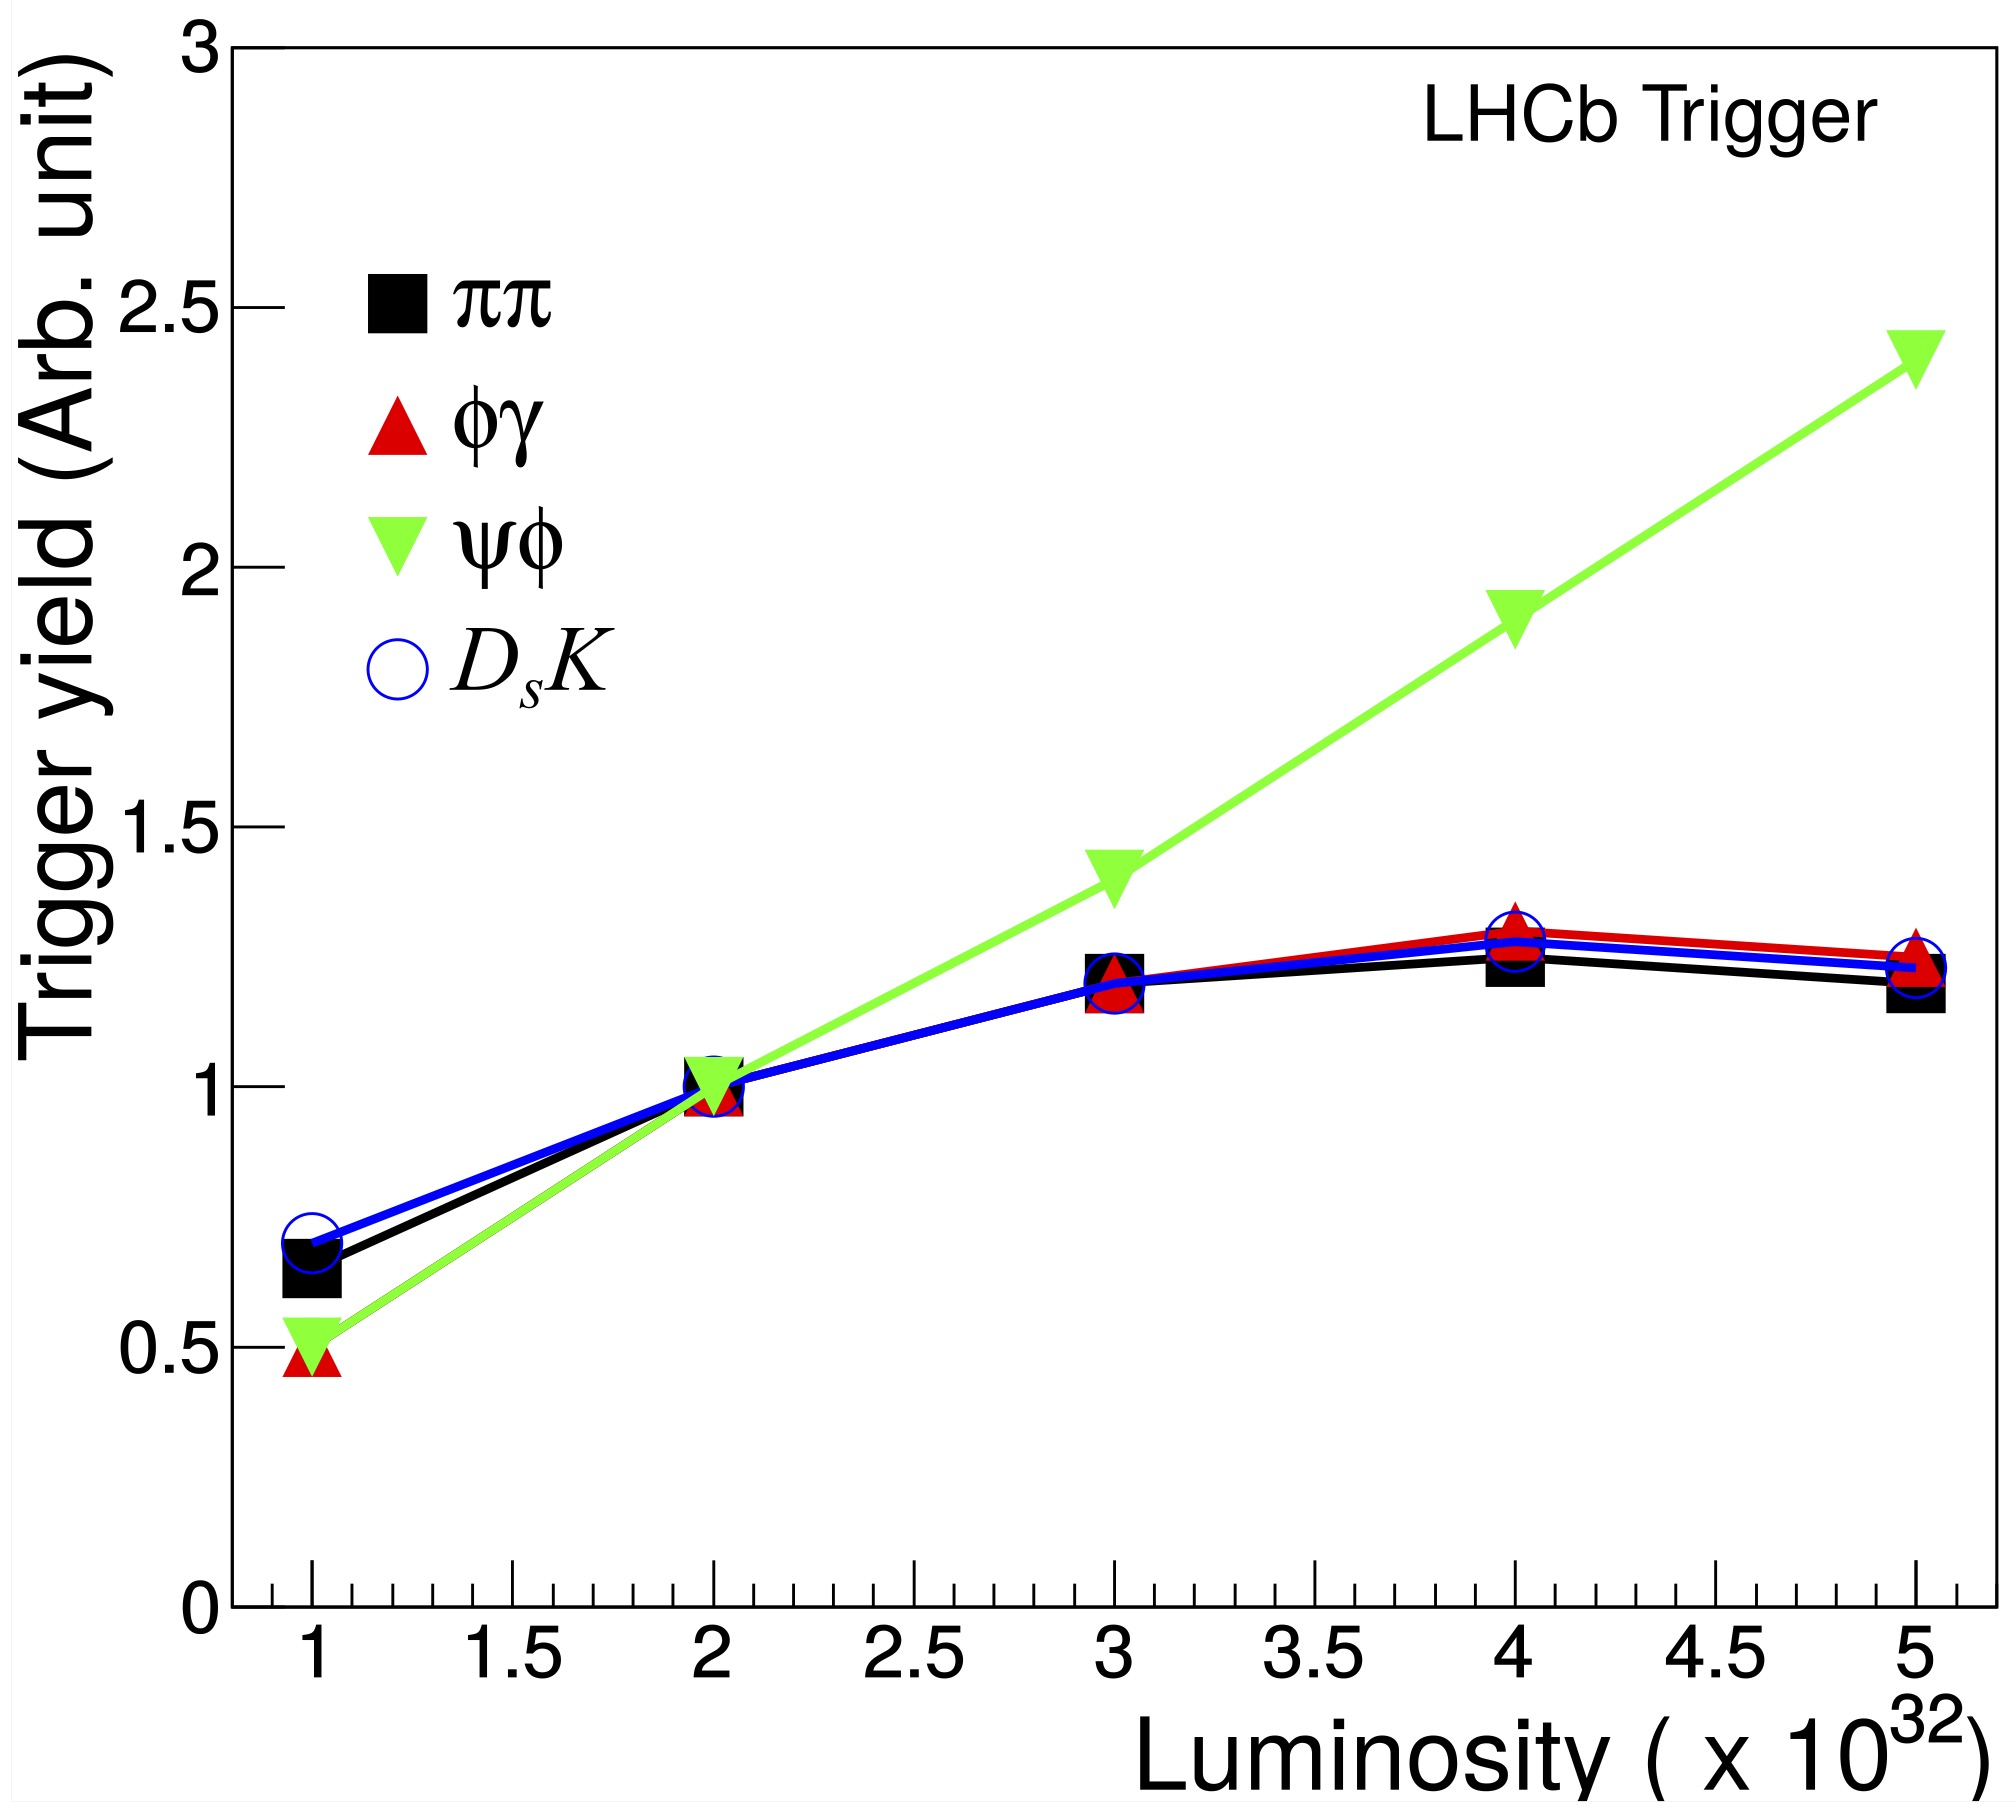
\includegraphics[width=\textwidth]{./dijkstra.png}
  \end{column}
  \begin{column}{.4\textwidth}
    \begin{alertblock}{what doesn't work}
    \begin{itemize}
        \item increased luminosity
        \item[$\rightarrow$] events passing hardware trigger
        \item[$\rightarrow$] saturating bandwidth
        \item[$\rightarrow$] tighten thresholds
        \item[$\rightarrow$] loss in efficiency
        \item[$\Rightarrow$] no increase in statistics for analyses
        \newline (depending on the decay channel)
    \end{itemize}
  \end{alertblock}
  \end{column}
  \end{columns}
  %data pile, dijkstra plot PID plot
\end{frame}

\begin{frame}
  \frametitle{removal of hardware trigger II}
  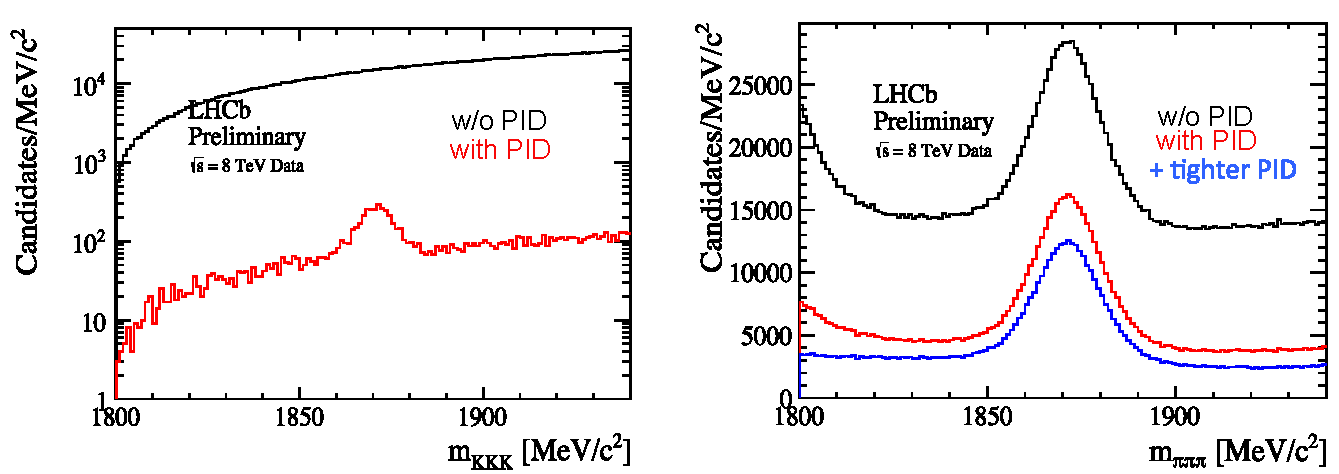
\includegraphics[width=\textwidth]{./stor.pdf}
  \begin{itemize}
      \item backgrounds from real physics events
      \item cannot distinguish signal from background w/o RICH PID
      \item[$\Rightarrow$] even selection in software
  \end{itemize}
\end{frame}

\begin{frame}
  \frametitle{ }
  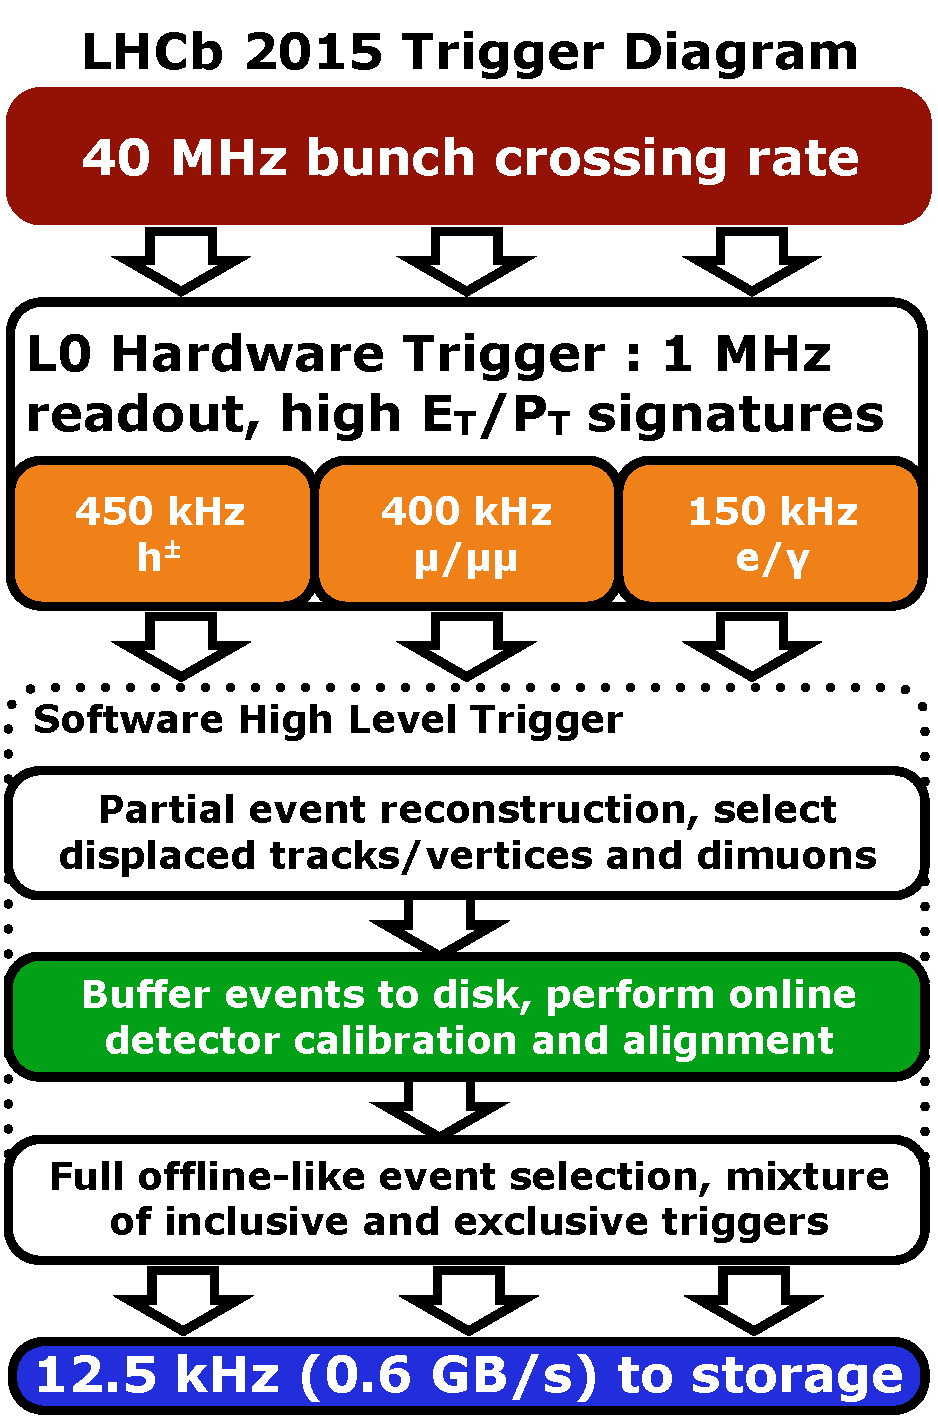
\includegraphics[width=.45\textwidth]{./LHCb_Trigger_RunII_May2015.pdf}
  \hspace{.01\textwidth}
  $\Rightarrow$
  \hspace{.01\textwidth}
  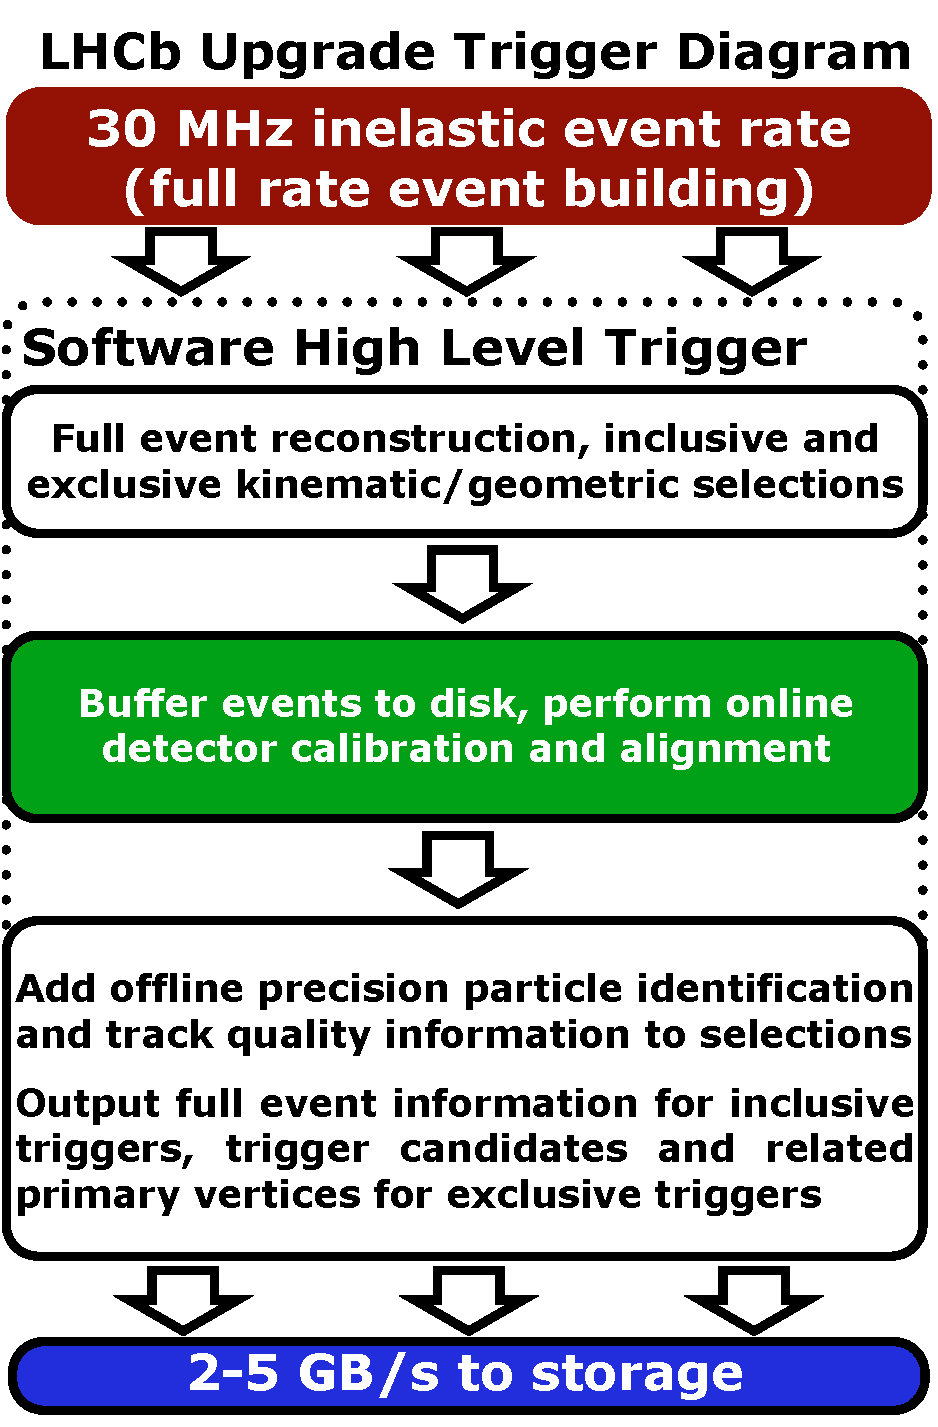
\includegraphics[width=.45\textwidth]{./LHCb_Trigger_RunIII_May2015.pdf}
\end{frame}

\begin{frame}[t]
  \frametitle{Luxury problem: MHz signals}
  
\includegraphics[width=.6\textwidth]{./pile.pdf}
  \only<1>{
  \begin{itemize}
    \item Selecting and storing full events could work for rare signal
    \item When dealing with ``millions'' of good signal events, rejecting background isn't enough to stay within processing bandwidths
  \end{itemize}
}
\only<2>{
  \begin{exampleblock}{The TURBO approach}
    \begin{itemize}
        \item once a decay is reconstructed (mass, decay time, Dalitz plot)
          \newline no need to access raw data for analysts
        \item once a decay is reconstructed in the trigger
          \newline no need to re-reconstruct offline

        \item (unaffordable to study raw data for millions of events anyway)
    \end{itemize}
  \end{exampleblock}
}
\end{frame}

\begin{frame}
  \frametitle{store what you need}
  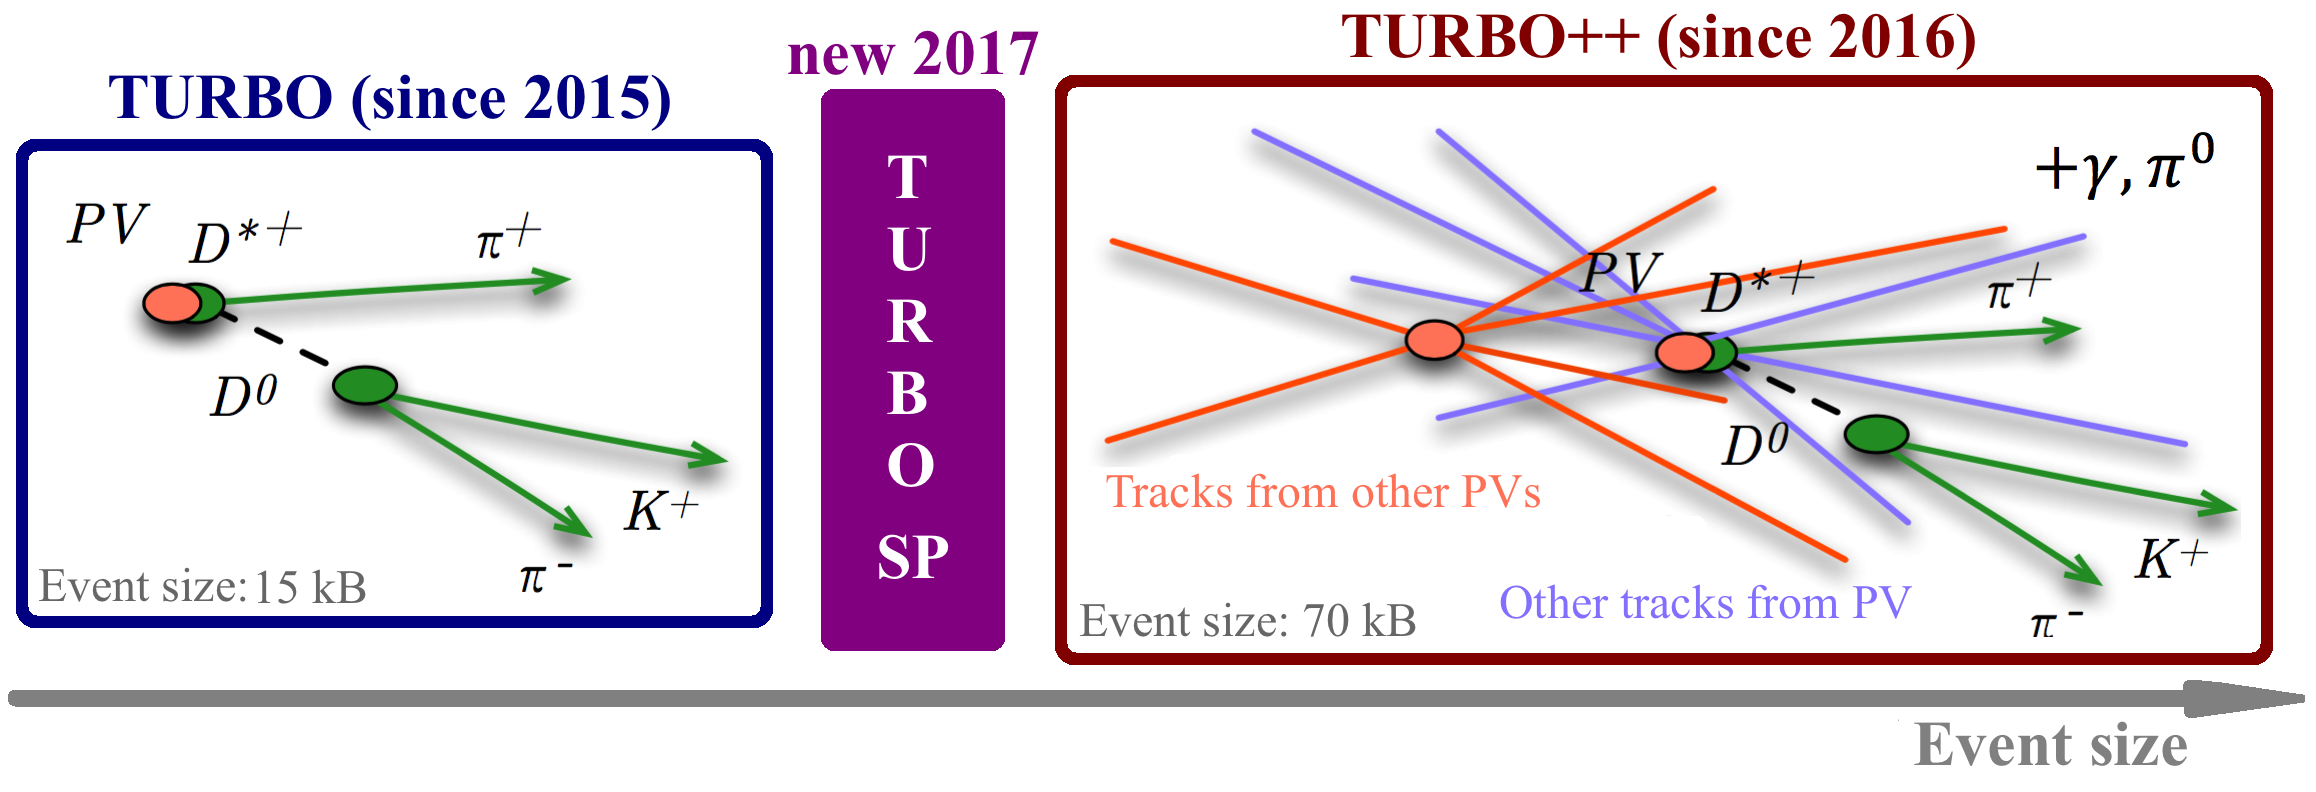
\includegraphics[width=.8\textwidth]{./turbosp-002.png}

  {\footnotesize{\texttt{10.1016/j.cpc.2016.07.022}}}
  
  \begin{block}{per trigger line storage definition}
  \begin{itemize}
      \item only decay and nothing else
      \item decay and selected reconstructed objects
      \item all \emph{reconstructed} objects (no raw data)
      \item full raw event
  \end{itemize}
  TURBO triggers must be a default for many analyses
  \end{block}
\end{frame}

\begin{frame}
  \frametitle{Bandwidth division I}
  \begin{itemize}
    \item There's always an efficiency vs. event rate tradeoff
    \item assume: every analysis could max out the full data bandwidth to maximise their \emph{efficiency}
    \item compromises need to be made
    \item ideally with little \emph{sensitivity} loss
  \end{itemize}

  \begin{block}{}
    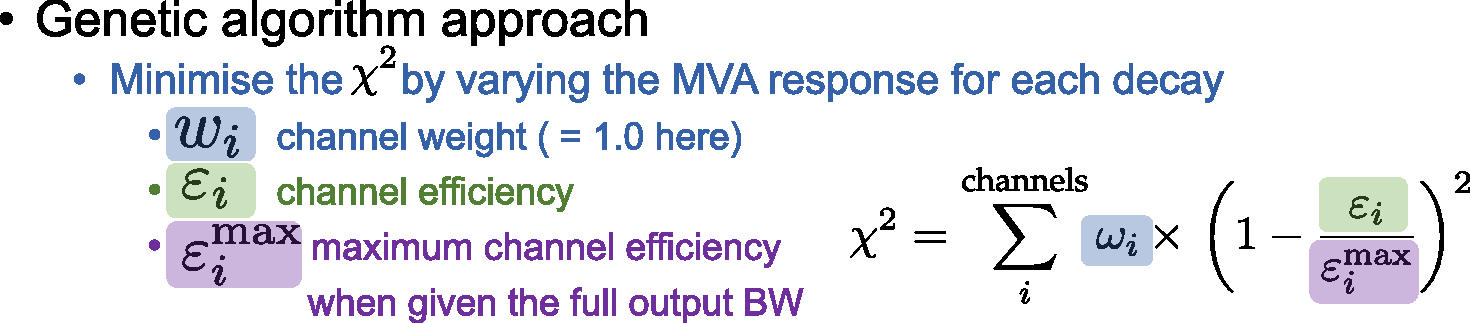
\includegraphics[width=\textwidth]{./BW.pdf}
    \begin{itemize}
        \item if sum of all channels exceeds total bandwidth \newline$\rightarrow$ assume random dropping of events
    \end{itemize}
  \end{block}


{\footnotesize{\texttt{LHCb-PUB-2017-006}}}
\end{frame}

\begin{frame}
  \frametitle{Bandwidth division II}
  \begin{columns}
    \begin{column}{.5\textwidth}
  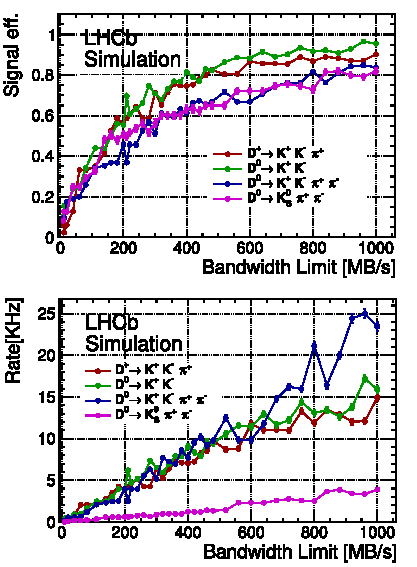
\includegraphics[width=\textwidth]{./BW-trend.pdf}
    \end{column}
    \begin{column}{.5\textwidth}
      going from maximal bandwidth to restricted bandwidth
      \begin{itemize}
      \item only small efficiency decrease
      \item ``90\,\% of the data holds 95\,\% of the statistical power''
      \end{itemize}
    \end{column}
    \end{columns}
  \end{frame}

\begin{frame}
  \frametitle{``Moore doesn't obey Moore's law''}

  \begin{columns}
    \begin{column}{.5\textwidth}
  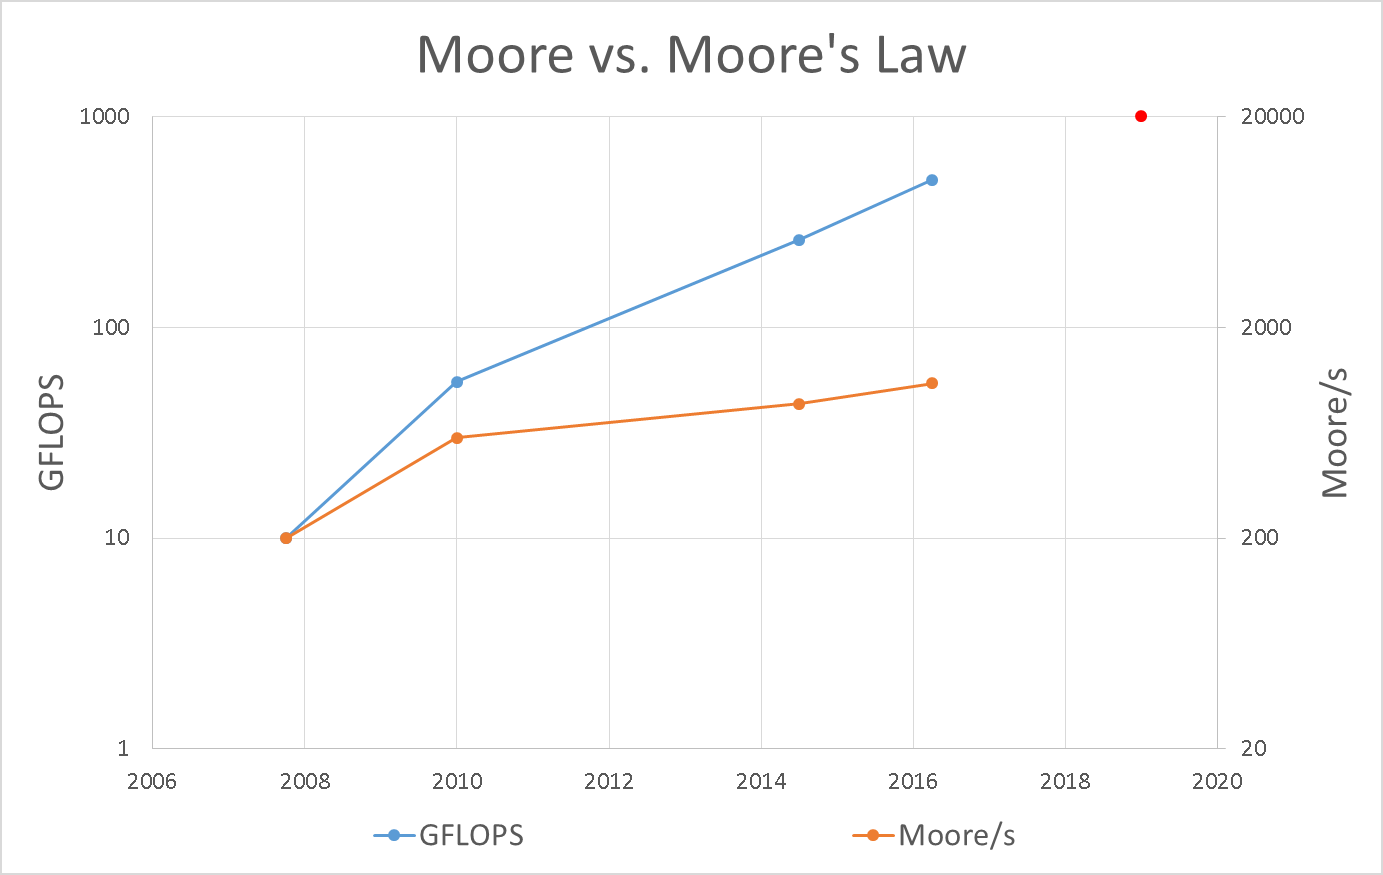
\includegraphics[width=\textwidth]{./moore.png}
    \end{column}
    \begin{column}{.5\textwidth}

  \begin{itemize}
    \item theoretical computing power of CPUs increases (per second, per Watt, per CHF)
    \item observed computed trigger decisions does not follow that increase
  \end{itemize}
    \end{column}
    \end{columns}
    \begin{alertblock}{reasons from a CPU's point of view \only<2>{II}\only<1>{I}/II}
    \only<1>{
  \begin{itemize}
    \item modern vector units process 2, 4, or 8 inputs at a time
      \newline$\leadsto$ our software often didn't use these
      \newline$\rightarrow$ 7/8 of the silicon unused!
  \end{itemize}
    }
    \only<2>{
  \begin{itemize}
    \item software not parallelised (just start multiple processes on a multicore machine)
    \newline$\leadsto$ processes compete for memory
    \newline$\leadsto$ even multiple instances of the same data (detector geometry)
    \newline$\rightarrow$ CPU waits for data instead of computing
  \end{itemize}
    }
\end{alertblock}

\end{frame}

\begin{frame}
  overview tracking (stages and types)
\end{frame}

\begin{frame}
  parametrised kalman
\end{frame}

\begin{frame}
  vectorised kalman
\end{frame}

\begin{frame}
  soa/aos
\end{frame}

\begin{frame}
  ghost prob
\end{frame}

\begin{frame}
  threadded brunel
\end{frame}

\begin{frame}
  WG production
\end{frame}

\begin{frame}
  conclusion
\end{frame}

\end{document}
